\documentclass[pdf]{beamer}
\usetheme{Berlin}
\setbeamertemplate{footline}[frame number]
\setbeamertemplate{section in toc}[sections numbered]
\setbeamertemplate{navigation symbols}{} 
\usepackage{graphicx}
\usepackage{appendixnumberbeamer}
\renewcommand{\arraystretch}{1.5}

\title{The Chinese Head Tax and Chinese Immigration to Canada}
\author{Amy Kim}
\date{October 11, 2022}

\begin{document}
\begin{frame}[plain]
    \titlepage
\end{frame}

\begin{frame}[plain]{Research Question}
    How did the Chinese Head Tax affect selection into immigration and/or immigrant wealth of Chinese immigrants to Canada in the early 20th century?    
\end{frame}

\begin{frame}[plain]{Outline}
    \tableofcontents
\end{frame}

\AtBeginSection[ ]
{
\begin{frame}[plain]{Outline}
    \tableofcontents[currentsection]
\end{frame}
}

% BACKGROUND
\section{Background}
\begin{frame}{Timeline}
    \begin{itemize}
        \item Early 1880s: Influx of Chinese immigrants for construction of Canadian Pacific Railway
        \item 1885: Chinese Exclusion Act institutes \$50 (~1.5k USD) tax
        \begin{itemize}
            \item Only exceptions for students, merchants, and diplomats
            \item Was not applied retroactively, but the tax was required even for re-entry going forward
            \item Failure to pay would result in being sent back to China -- many immigrants had to borrow money or enter indentured servitude contracts
        \end{itemize}
        \item 1900: Tax raised to \$100 (~3.5k USD)
        \item 1903: Tax raised to \$500 (~16k USD)
        \item 1923: Chinese immigration banned completely (with very few exceptions)
    \end{itemize}
\end{frame}

% DATA
\section{Data}
\begin{frame}[label = datasources]
    \frametitle{Data Sources}
    \centering
    \begin{itemize}
        \item Canadian Census \hyperlink{cancensus}{\beamerbutton{Details on Canadian Census}}
        \begin{itemize}
            \item Currently: at least 5\% sample from 1881-1921
            \item Entire Full-Count Data? \hyperlink{censustweet}{\beamerbutton{See Tweet}}
            \item Missing: mid-decade arrivals who exited before subsequent census
        \end{itemize}
        \item Chinese Registry 
        \begin{itemize}
            \item \textbf{Full count} of every person of Chinese origin arriving in Canada from 1885-1949
            \item Missing: full count of pre-1885 arrivals
        \end{itemize}
        \item US Census 
        \begin{itemize}
            \item For now, just a point of comparison
            \item Full count data from IPUMS from 1850-1940
            \item Missing: income/wealth data
        \end{itemize}
    \end{itemize}
    
\end{frame}

\begin{frame}[label = summstats]
	\frametitle{Chinese Immigrants Summary Statistics by Data Source}        
    \centering 
	\begin{table}[H]
		\resizebox{\textwidth}{!}{
            % latex table generated in R 4.0.3 by xtable 1.8-4 package
% Mon Oct 10 23:48:19 2022
\begin{tabular}{lccc}
  \hline
 & CA Census (1901-1921) & Chinese Registry (1885-1924) & US Census (1900-1920) \\ 
  \hline
\% Male & 0.98 & 0.98 & 0.95 \\ 
   & (0.16) & (0.15) & (0.21) \\ 
  \% Married & 0.55 & - & 0.44 \\ 
    & (0.5) & - & (0.5) \\ 
  Avg. Age at Imm & 23.20 & 25.95 & 20.92 \\ 
     & (8.99) & (21.86) & (9.78) \\ 
  \% Can Read & 0.68 & - & 0.77 \\ 
        & (0.47) & - & (0.42) \\ 
  \% Labourers & 0.20 & 0.62 & 0.32 \\ 
           & (0.4) & (0.48) & (0.47) \\ 
   \hline
Obs &   4230 &  90946 & 186523 \\ 
   \hline
\end{tabular}

		}
	\end{table}  
    \hyperlink{summstatscensus}{\beamerbutton{Summ. Stats by Group in CA Census}}
\end{frame}


% INITIAL DESCRIPTIVES
\section{Initial Descriptives}
\begin{frame}[label = yrimmchi]{Chinese Immigration to Canada by Year and Data Source}
    \centering
    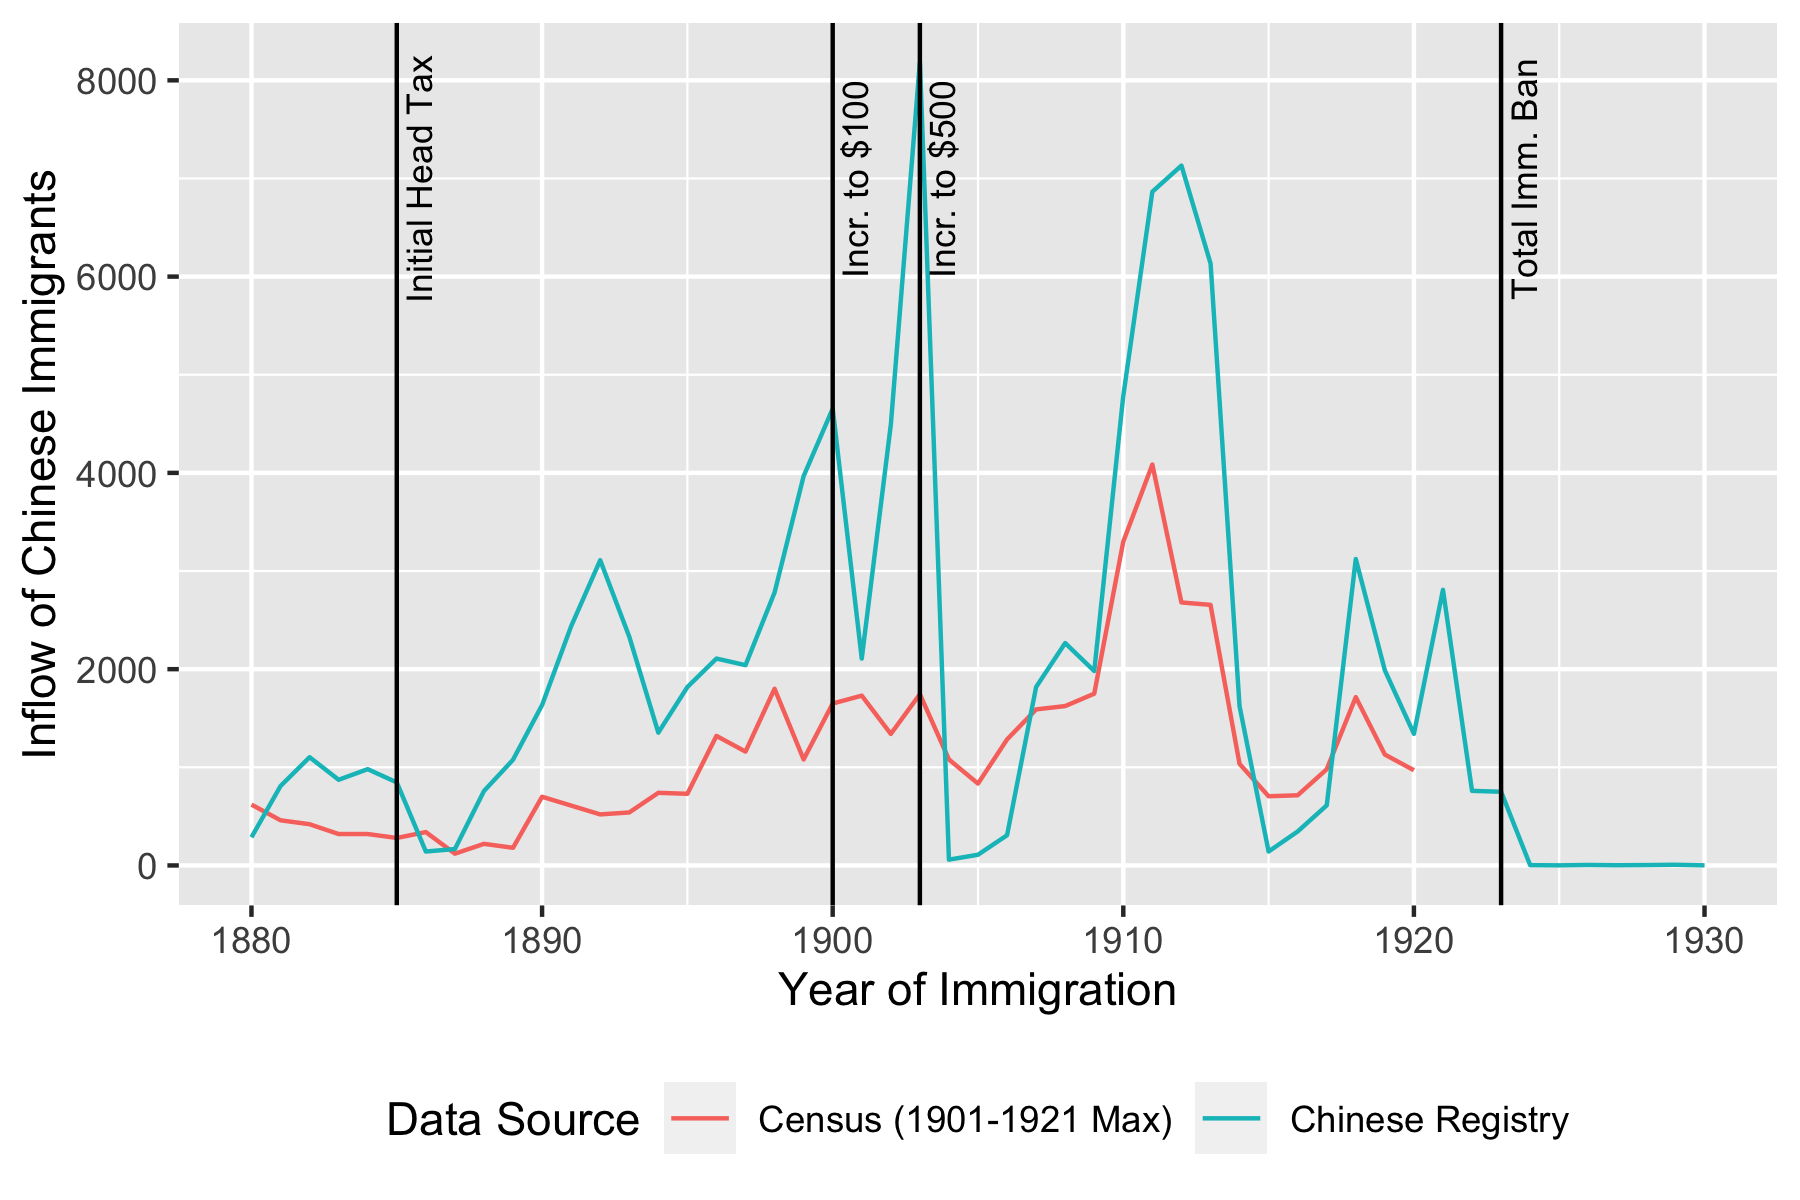
\includegraphics[width = 0.9\textwidth]{../../figs/yrimmchi_maxes.png}
    \hyperlink{taxespaid}{\beamerbutton{Avg Taxes Paid}}
    \hyperlink{taxbyyear}{\beamerbutton{\% Taxpayers by Year}}
    \hyperlink{dateimmchi}{\beamerbutton{Denisty by Year}}
    \hyperlink{yrimmchi_means}{\beamerbutton{Alt. Calculation}}
    \hyperlink{events1912}{\beamerbutton{Events in 1910s}}
\end{frame}

\begin{frame}[label = yrimmchius]{Chinese Immigration to Canada vs. US}
    \centering
    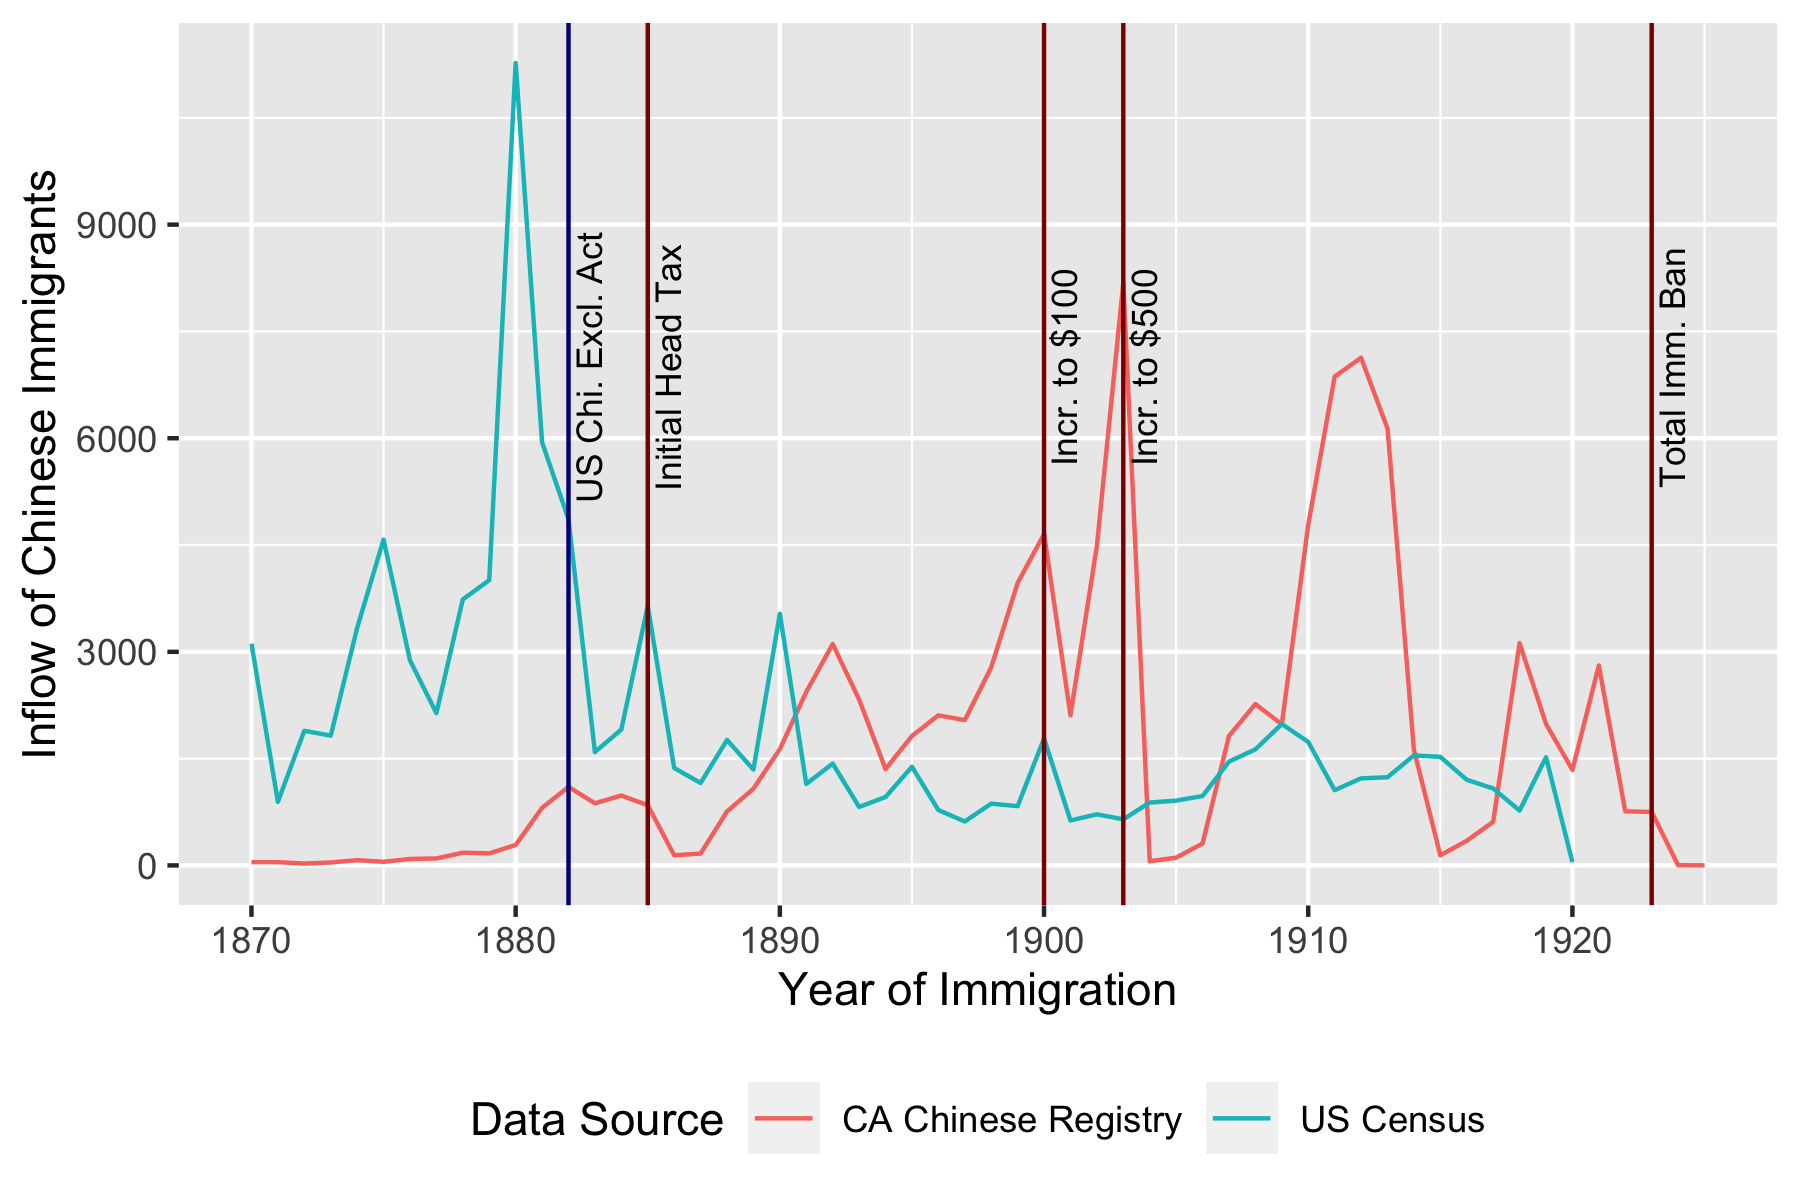
\includegraphics[width = 0.9\textwidth]{../../figs/yrimmchi_us.png}
    \hyperlink{yrimm_us}{\beamerbutton{All Immigration to US vs. Canada}}
    \hyperlink{yrimmall}{\beamerbutton{Immigration to Canada by Country}}
\end{frame}


\begin{frame}{Chinese Immigration by Occupation Group}
    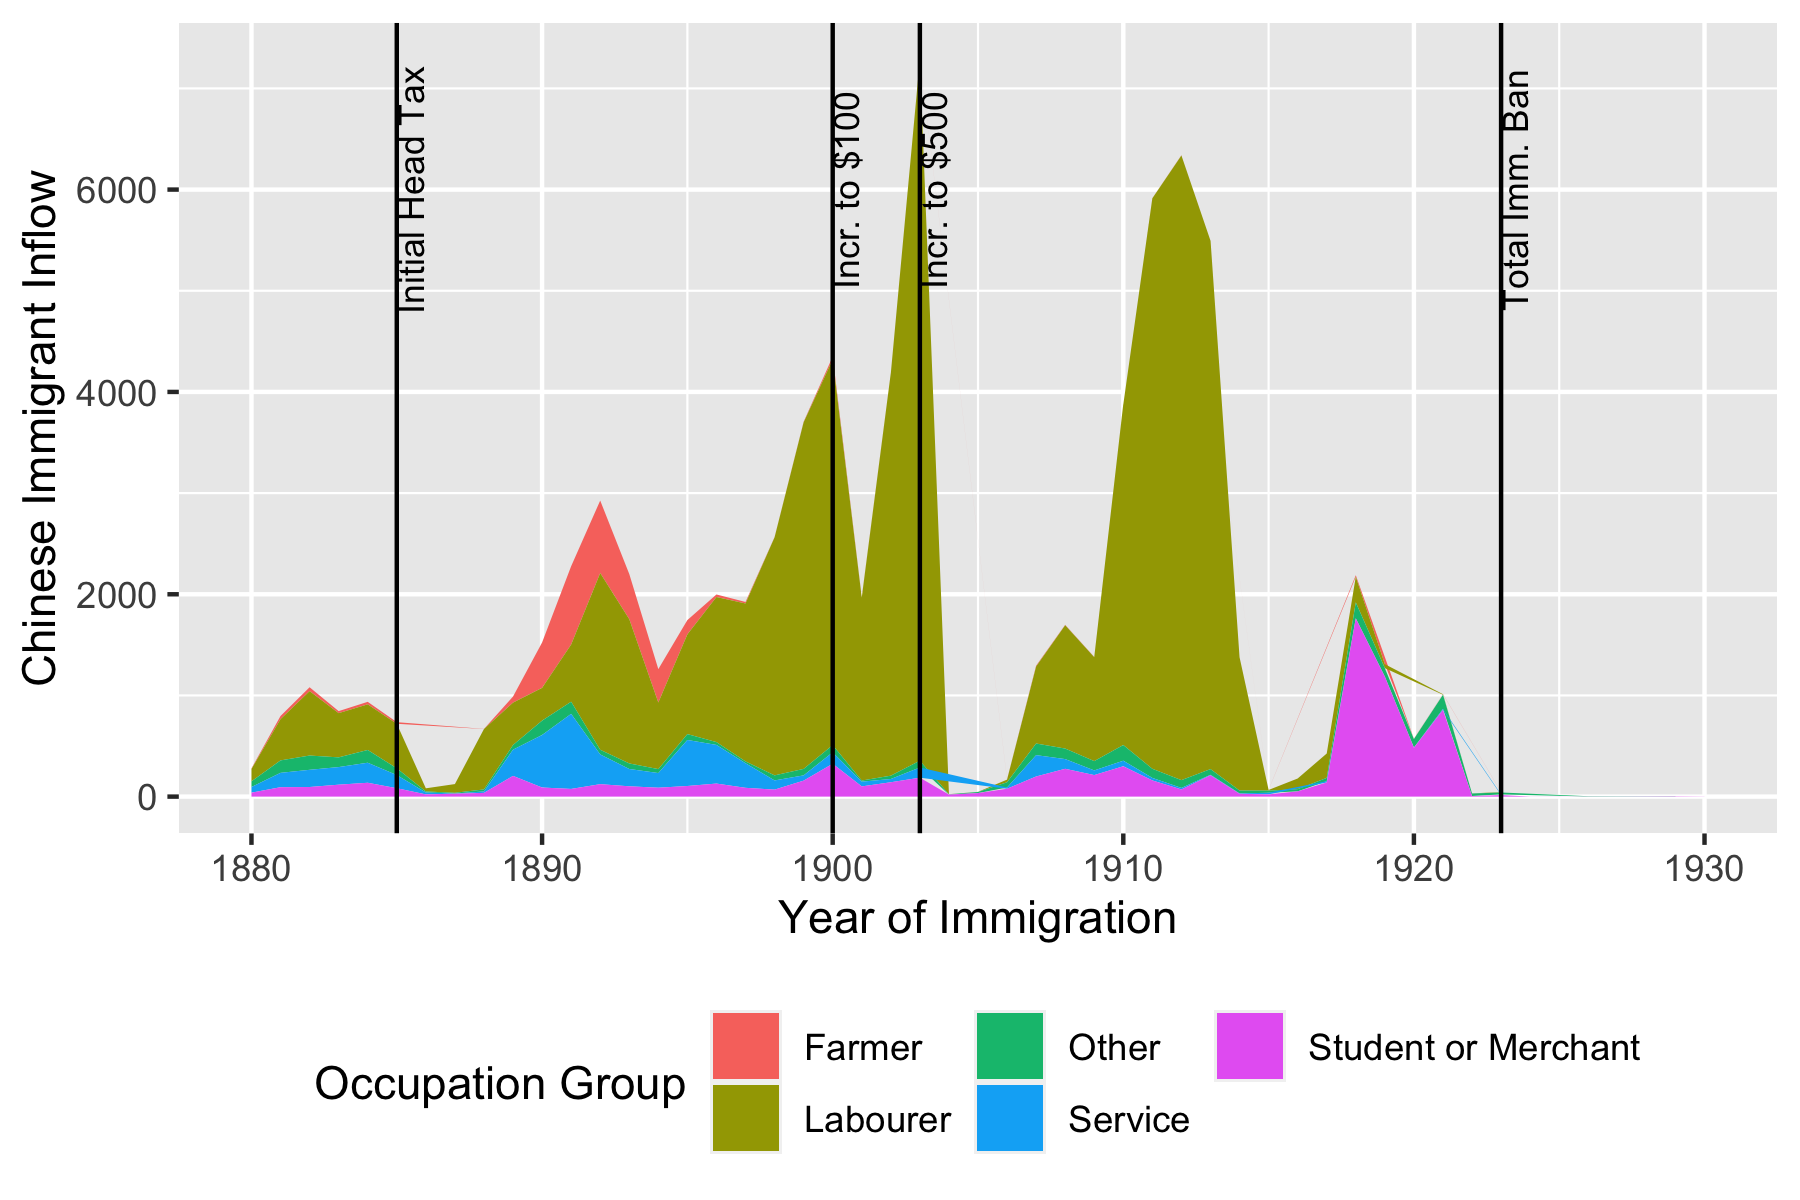
\includegraphics[width = \textwidth]{../../figs/chiocc.png}
\end{frame}

%%%%%%%%%%%%%%%%%%%%%%%%%%%%%%%%%%%%%%%%%%%%%%%%%%%%%%%
%%%%%%%%%%      A  P  P  E  N  D  I  X      %%%%%%%%%%%
%%%%%%%%%%%%%%%%%%%%%%%%%%%%%%%%%%%%%%%%%%%%%%%%%%%%%%%
\appendix
%---------------------------
%  Details on sampling for currently publically available Canadian Census Data
%---------------------------
\renewcommand{\arraystretch}{1}
\begin{frame}[label = cancensus]
    \frametitle{Canadian Census Data}
    \centering
    \begin{tabular}{|r||c|c|}
        \hline 
        Year & Coverage & Sampling Method \\
        \hline 
        1852 & 20\% & Random, clustered sample \\
        1871 & 1.8\% & Stratified sample (8 strata)\\
        1881 & 100\% & Full sample \\
        1891 & 5\% & Random sample\footnote{Also includes 10\% of cities and 100\% of all large dwellings and some areas of Ontario} \\
        1901 & 5\% & \textit{Not Specified} \\
        1911 & 5\% & Random sample\footnote{Also includes 10\% of large dwellings and 25\% of multi-unit dwellings} \\
        1921 & 4\% & Random sample\footnote{Also includes 10\% of large dwellings and 20\% of multi-unit dwellings} \\
        \hline
    \end{tabular} \\
    Note: China was not listed as a country of origin in the data until the 1881 census.
    \hyperlink{datasources}{\beamerbutton{Back to Slides}}
\end{frame}

%---------------------------
%  Tweet on Census Data
%---------------------------
\begin{frame}[label=censustweet]
    \frametitle{Full-Count Canadian Census Data -- Coming Soon!}
    
\includegraphics[width = 0.9\textwidth]{../../figs/census_tweet.png}
    \hyperlink{datasources}{\beamerbutton{Back to Slides}}
\end{frame}

%---------------------------
%   Summary Statistics for Census by Group
%---------------------------
\begin{frame}[label = summstatscensus]
	\frametitle{Summary Statistics for by Group in Canadian Census}
	\begin{table}[H]
        \centering 
		\resizebox{0.6\textwidth}{!}{
            % latex table generated in R 4.0.3 by xtable 1.8-4 package
% Mon Oct 10 23:48:18 2022
\begin{tabular}{lccc}
  \hline
 & All & Immigrants & Chinese Imm \\ 
  \hline
\% Male & 0.52 & 0.58 & 0.98 \\ 
   & (0.5) & (0.49) & (0.16) \\ 
  \% Married & 0.37 & 0.54 & 0.55 \\ 
    & (0.48) & (0.5) & (0.5) \\ 
  Avg. Age & 26.61 & 34.64 & 34.79 \\ 
     & (19.5) & (17.81) & (11.74) \\ 
  \% Can Read & 0.84 & 0.91 & 0.68 \\ 
      & (0.36) & (0.28) & (0.47) \\ 
  Avg. Earnings & 734.9 & 783.7 & 441.6 \\ 
       & (12756.29) & (1212.1) & (296.33) \\ 
  \% Labourers & 0.03 & 0.05 & 0.20 \\ 
        & (0.16) & (0.21) & (0.4) \\ 
   \hline
Obs & 1004561 &  204777 &    4230 \\ 
   \hline
\end{tabular}

		}
	\end{table}  
    \hyperlink{datasources}{\beamerbutton{Back to Slides}}
\end{frame}

%---------------------------
%  Taxes Paid by Year
%---------------------------
\begin{frame}[label=taxespaid]
    \frametitle{Head Tax Payers: Average Taxes Paid by Year}
    \centering
    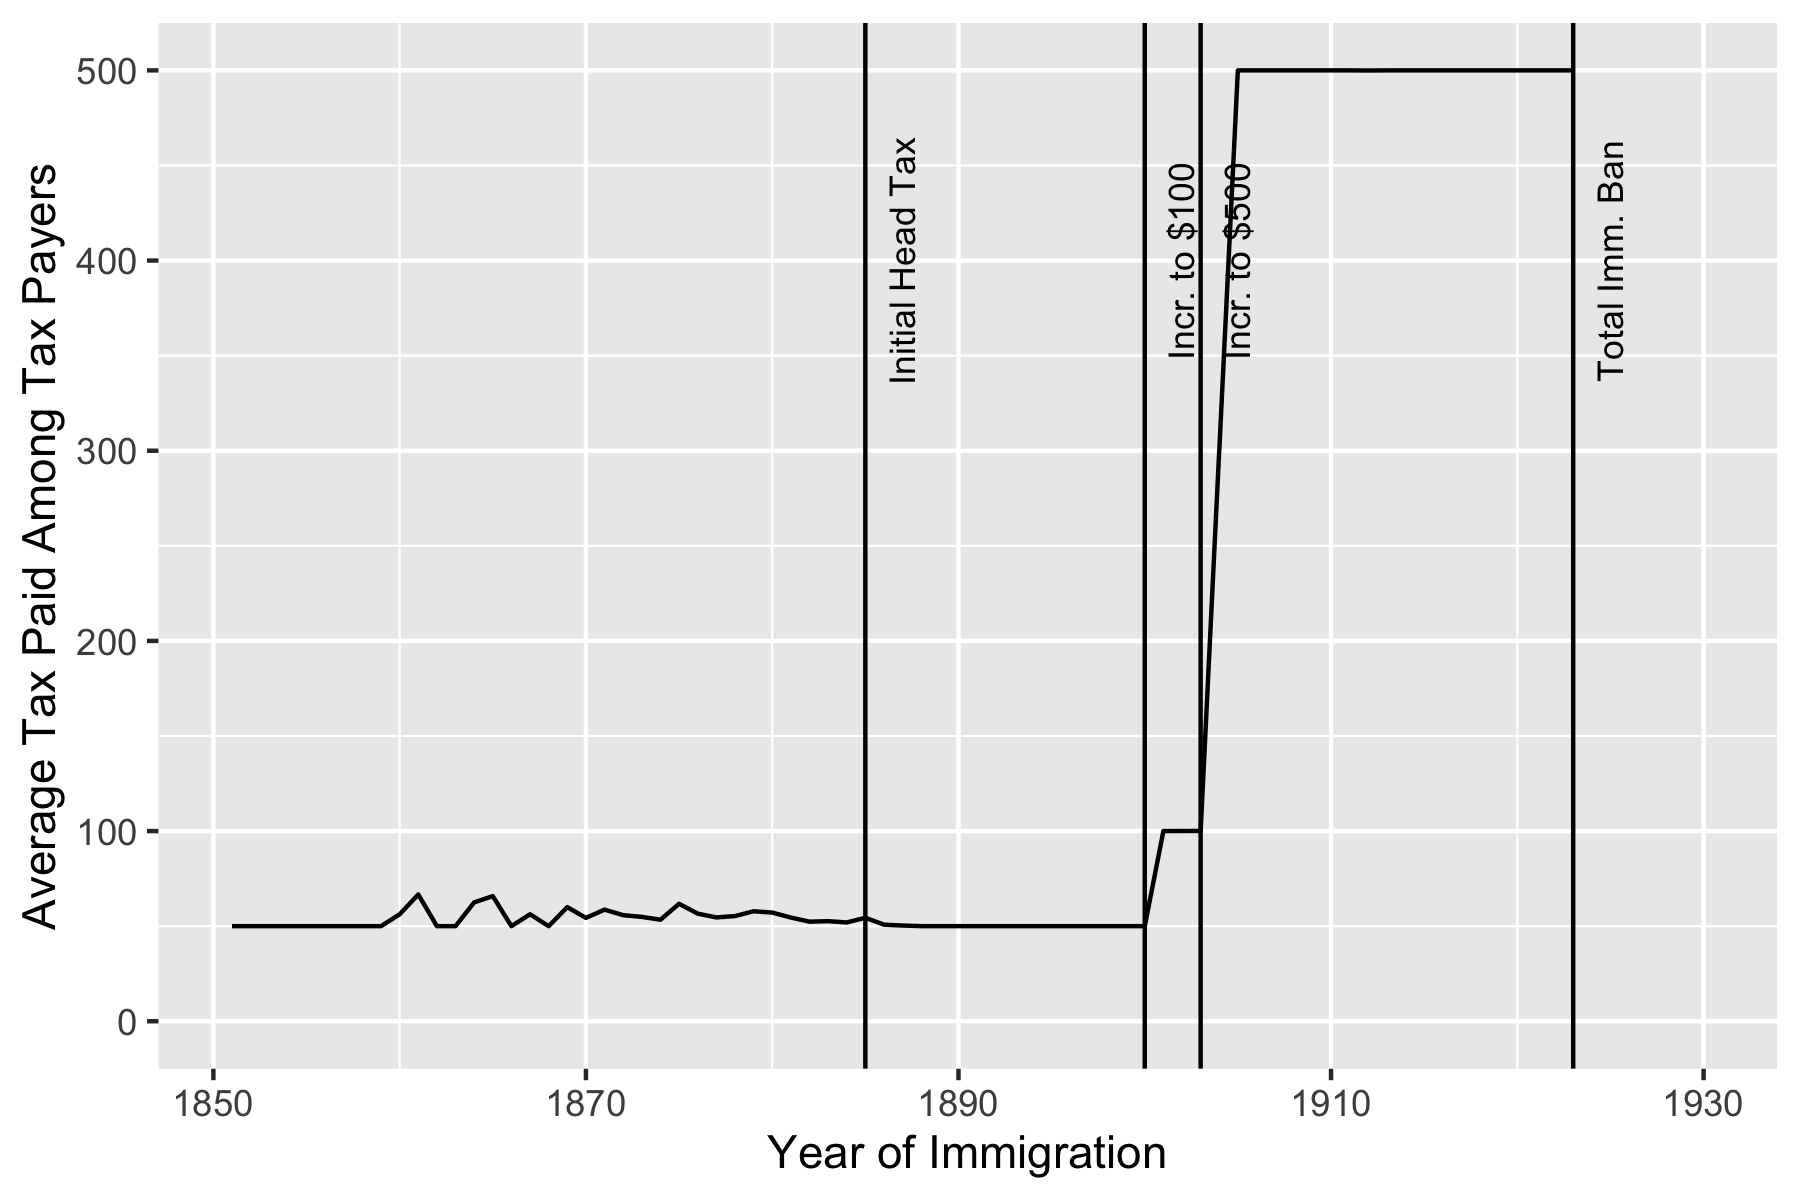
\includegraphics[width = 0.9\textwidth]{../../figs/taxespaid.png}
    \centering
    \hyperlink{yrimmchi}{\beamerbutton{Back to Slides}}
\end{frame}

%---------------------------
%  Taxpayers as % of Arrivals by Year
%---------------------------
\begin{frame}[label=taxbyyear]
    \frametitle{Taxpayers as \% of Arrivals by Year}
    \centering
    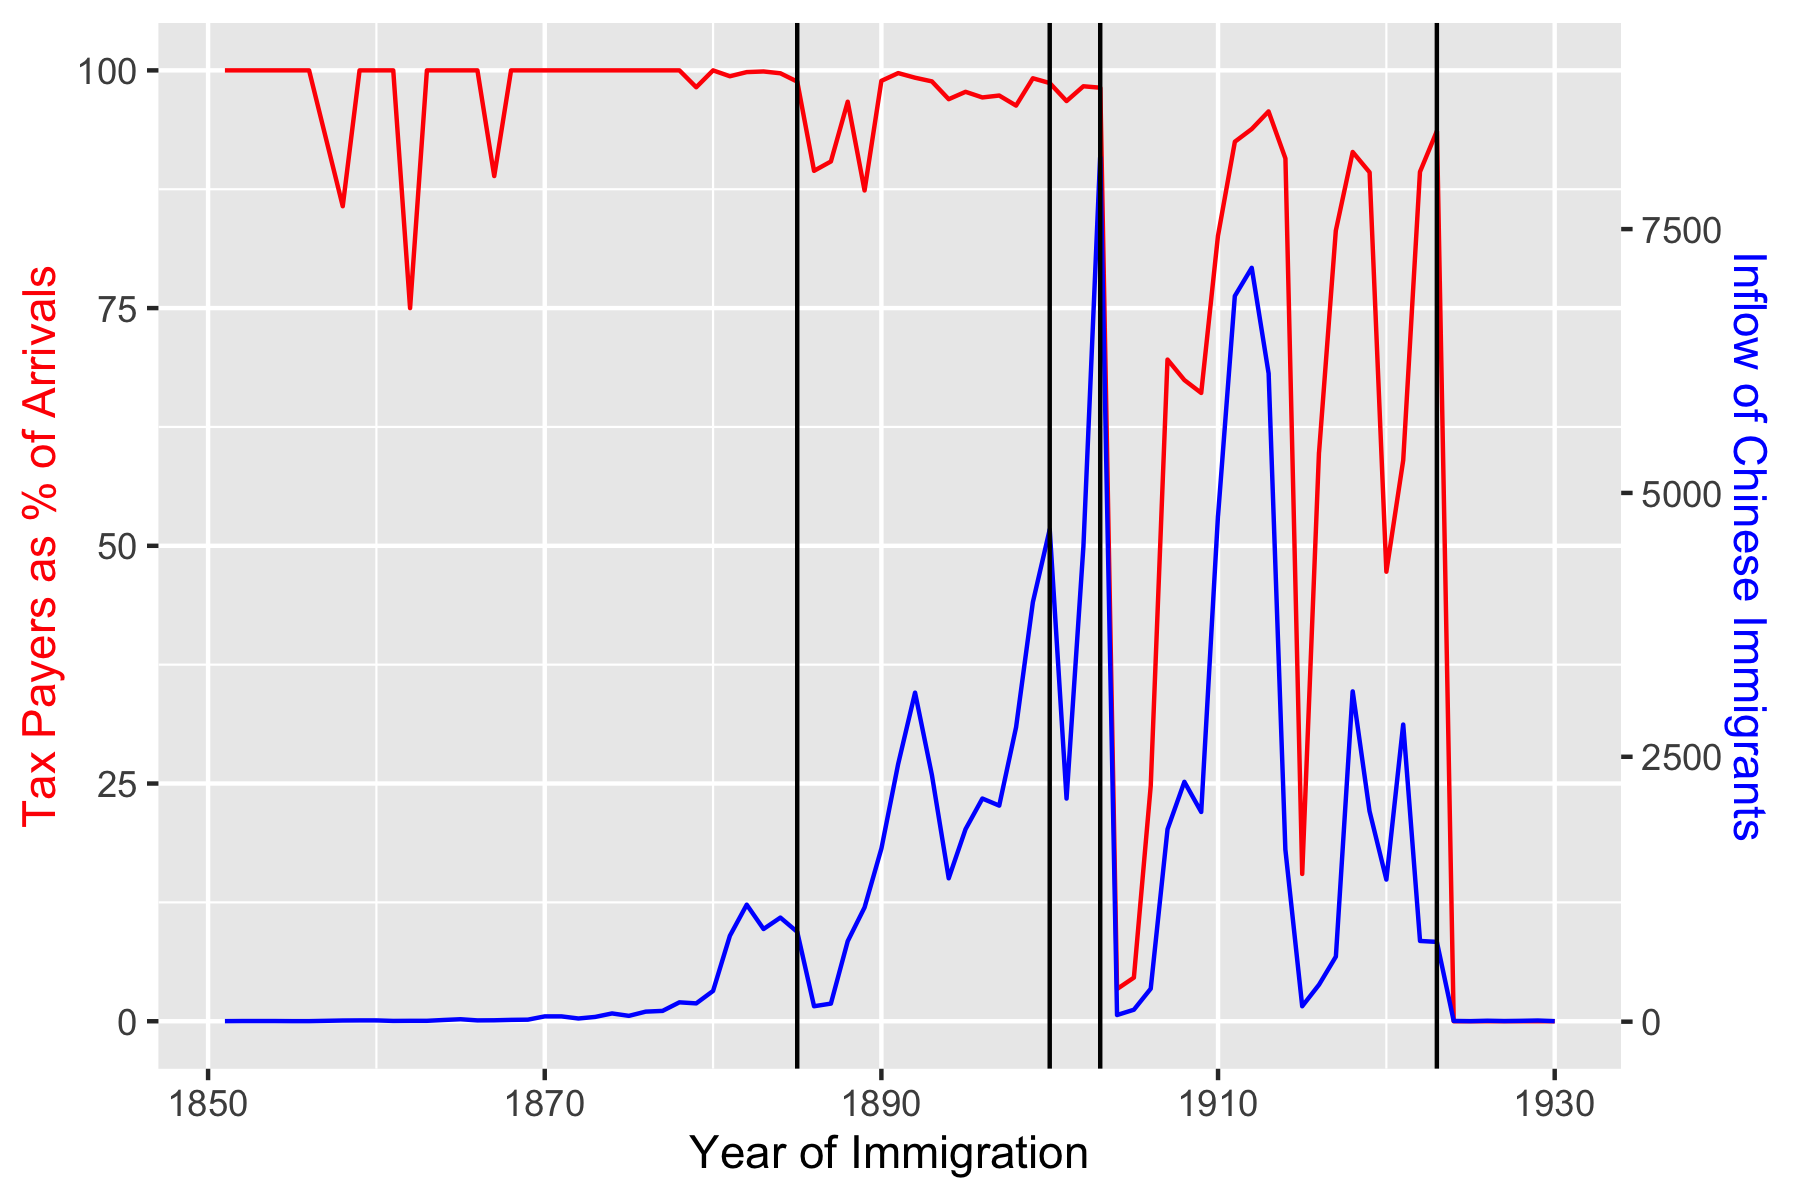
\includegraphics[width = 0.9\textwidth]{../../figs/taxbyyear.png}
    \hyperlink{yrimmchi}{\beamerbutton{Back to Slides}}
\end{frame}

%---------------------------
%  Chinese Immigration to Canada by Year and Data Source -- Using Census Means instead of Census Maxes
%---------------------------

\begin{frame}[label = yrimmchi_means]
	\frametitle{Density of Chinese Immigration to Canada by Date}
    \centering
	\begin{figure}[H]
		\begin{center}
			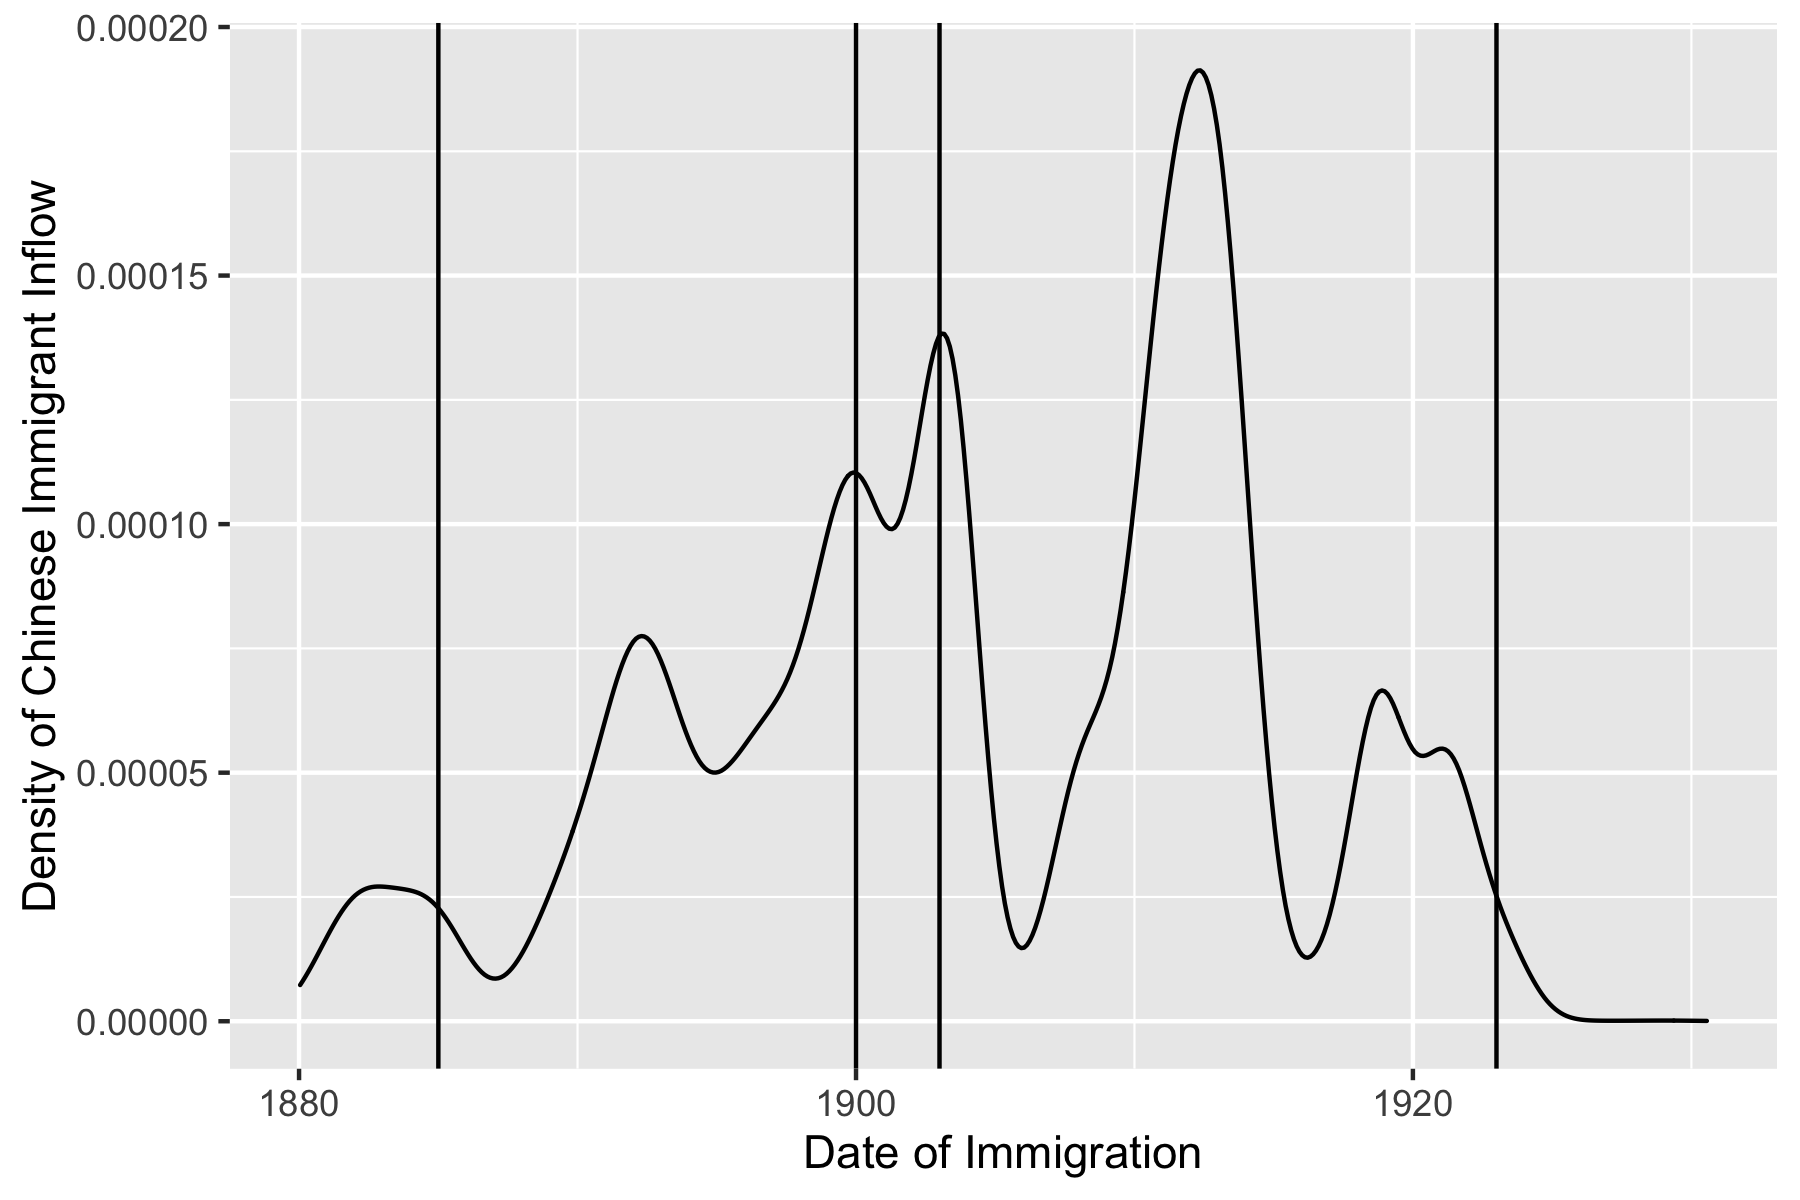
\includegraphics[width=0.9\textwidth]{../../figs/dateimmchi.png}
		\end{center}
	\end{figure}
    \hyperlink{yrimmchi}{\beamerbutton{Back to Slides}}
\end{frame}

%---------------------------
%   Density of Chinese Immigration to Canada by Date
%---------------------------

\begin{frame}[label = dateimmchi]
	\frametitle{Chinese Immigration to Canada Using Cross-Year Means for Census Data}
    \centering
	\begin{figure}[H]
		\begin{center}
			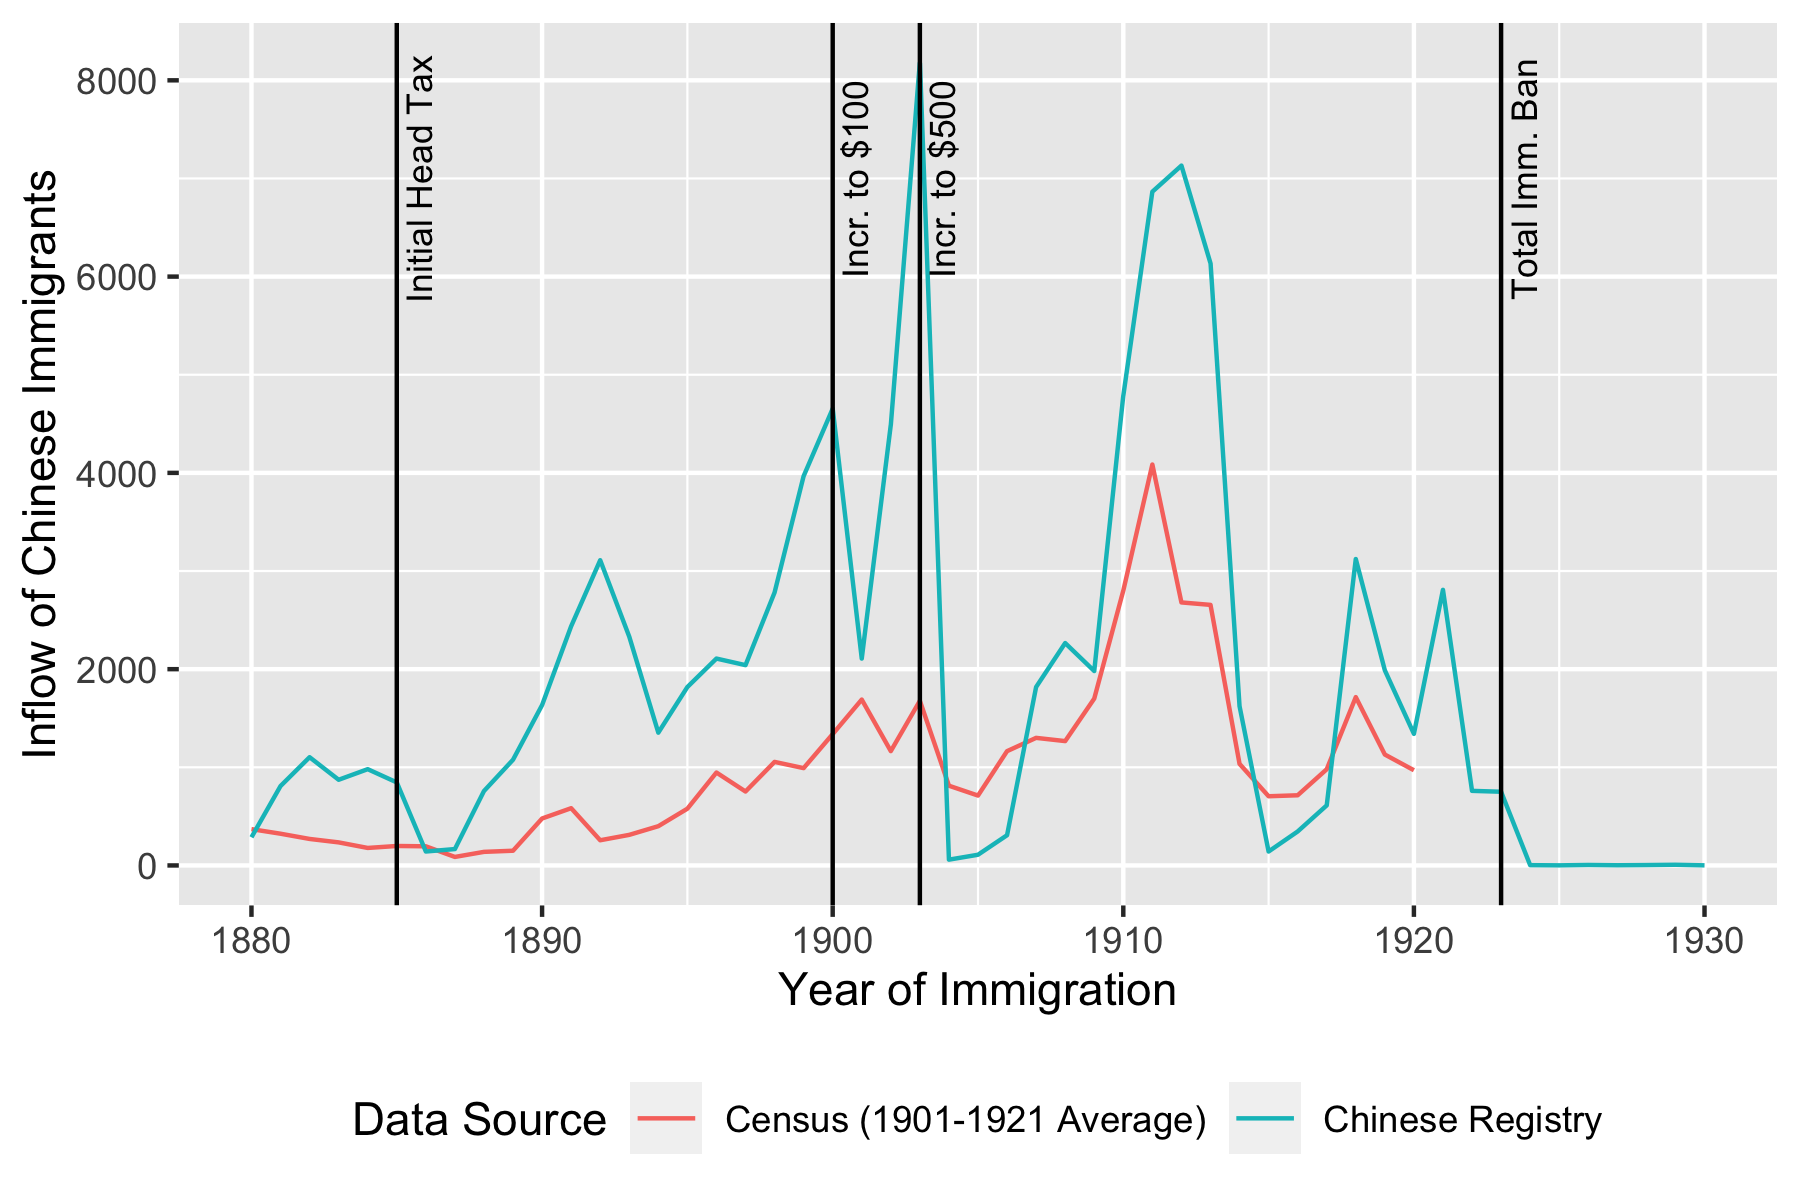
\includegraphics[width=0.9\textwidth]{../../figs/yrimmchi_means.png}
		\end{center}
	\end{figure}
    \hyperlink{yrimmchi}{\beamerbutton{Back to Slides}}
\end{frame}

%---------------------------
%   Major Events in 1910s
%---------------------------
\begin{frame}[label = events1912]
	\frametitle{Relevant Events in the 1910s}
	\begin{itemize}
        \item Canada [1910]: Immigration Act of 1910 further restricts immigration, not expands
        \item Canada [1912]: Head Tax Certificates reissued with photo 
        \begin{itemize}
            \item Unlikely to have such a massive spike just from using other people's certificates 
        \end{itemize}
        \item China: Republic of China established in 1912 following Xinhai Revolution (1911)
        \begin{itemize}
            \item If this is primary cause of spike, would expect some change in regional origin of Chinese immigrants \hyperlink{originchi}{\beamerbutton{Chinese Immigration by Origin by Year}}
            \item Also would not expect to see spike in immigration from other countries \hyperlink{yrimmall}{\beamerbutton{Immigration to Canada from Different Countries}}
        \end{itemize}
        \item Worldwide: WWI begins July 1914
        \begin{itemize}
            \item Unclear why most of spike is prior to 1914 -- general global unrest?
        \end{itemize}
    \end{itemize}
    \hyperlink{yrimmchi}{\beamerbutton{Back to Slides}}
\end{frame}

%---------------------------
%   Chinese immigration by Origin County
%---------------------------
\begin{frame}[label = originchi]
	\frametitle{Chinese Immigration by County of Origin in China}
    \centering
	\begin{figure}[H]
		\begin{center}
			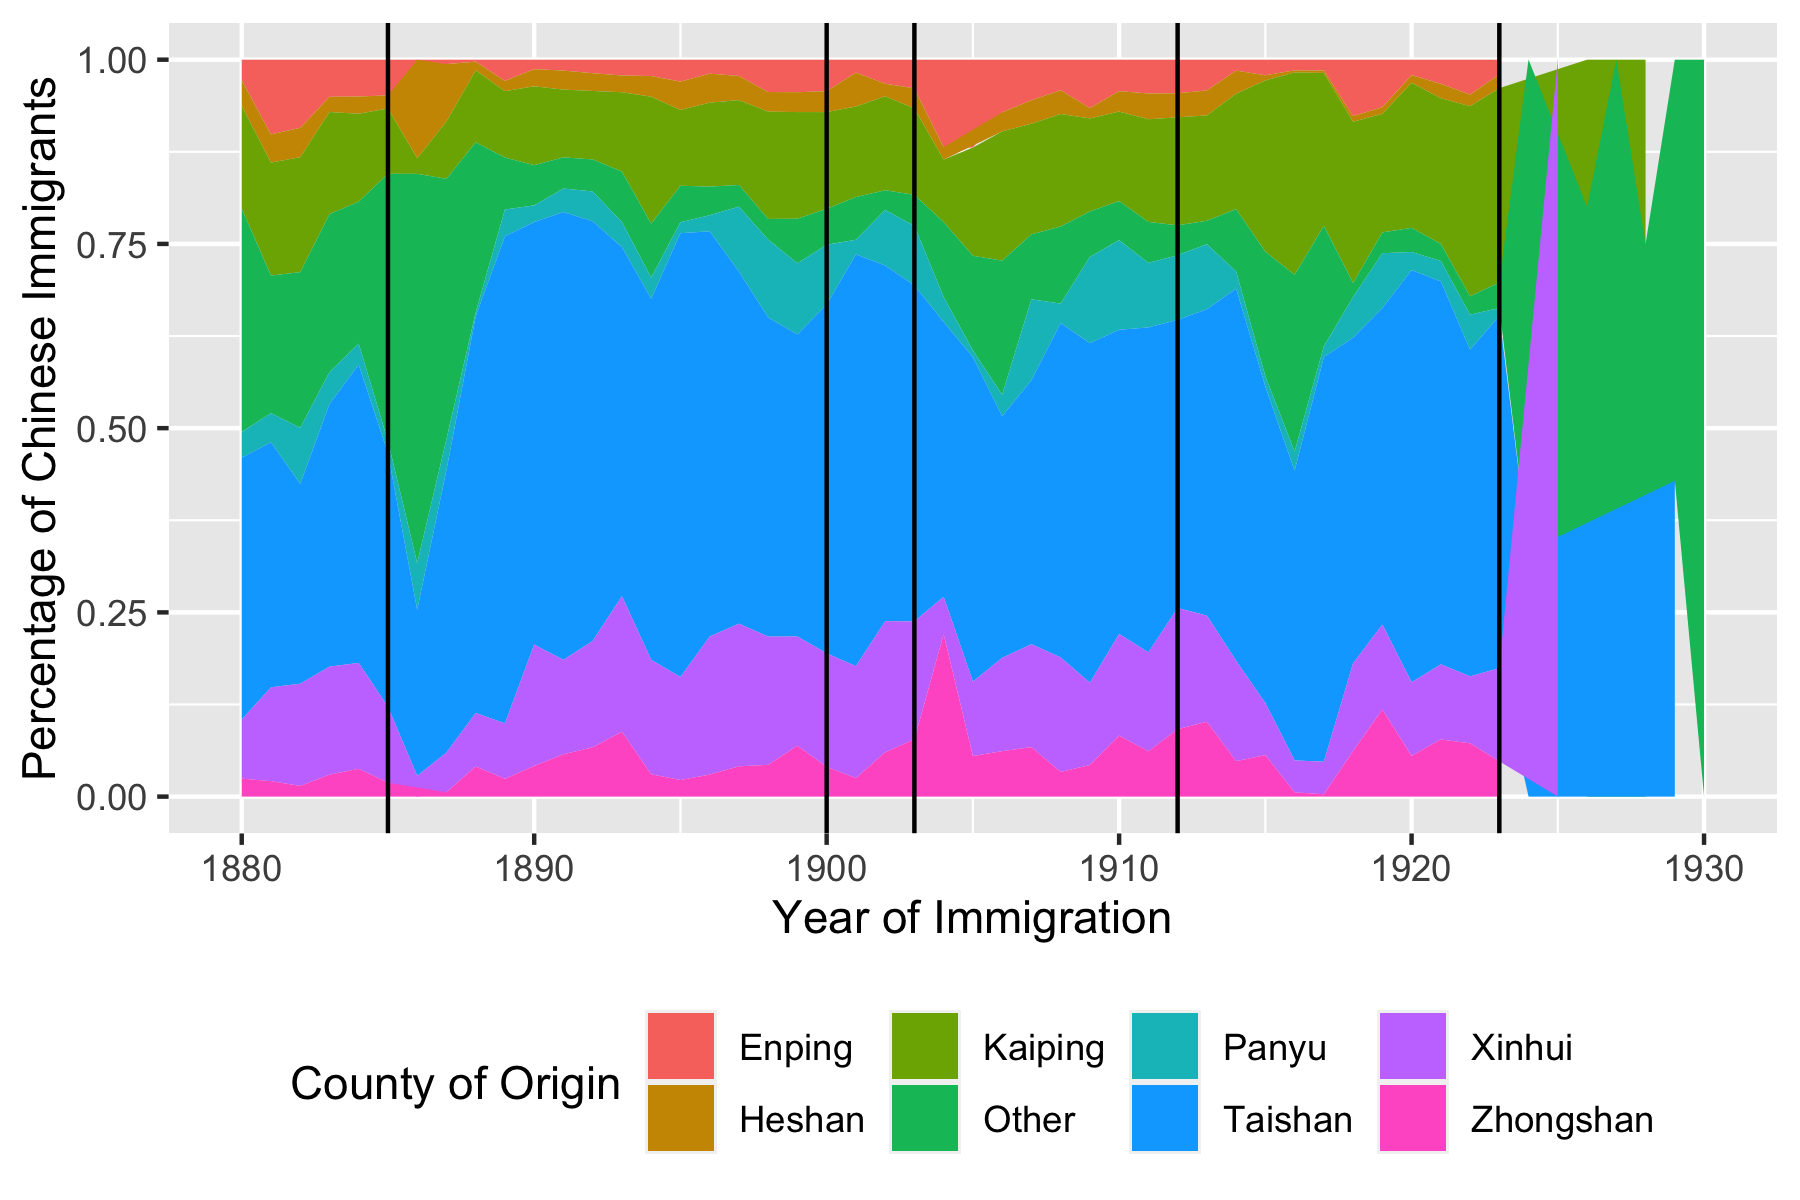
\includegraphics[width=0.9\textwidth]{../../figs/chiorig.png}
		\end{center}
	\end{figure}
    \hyperlink{events1912}{\beamerbutton{Back to 1910s Events}}
\end{frame}

%---------------------------
%  All Immigration to Canada vs. US
%---------------------------
\begin{frame}[label = yrimm_us]
	\frametitle{All Immigration to Canada vs. US}
    \centering
	\begin{figure}[H]
		\begin{center}
			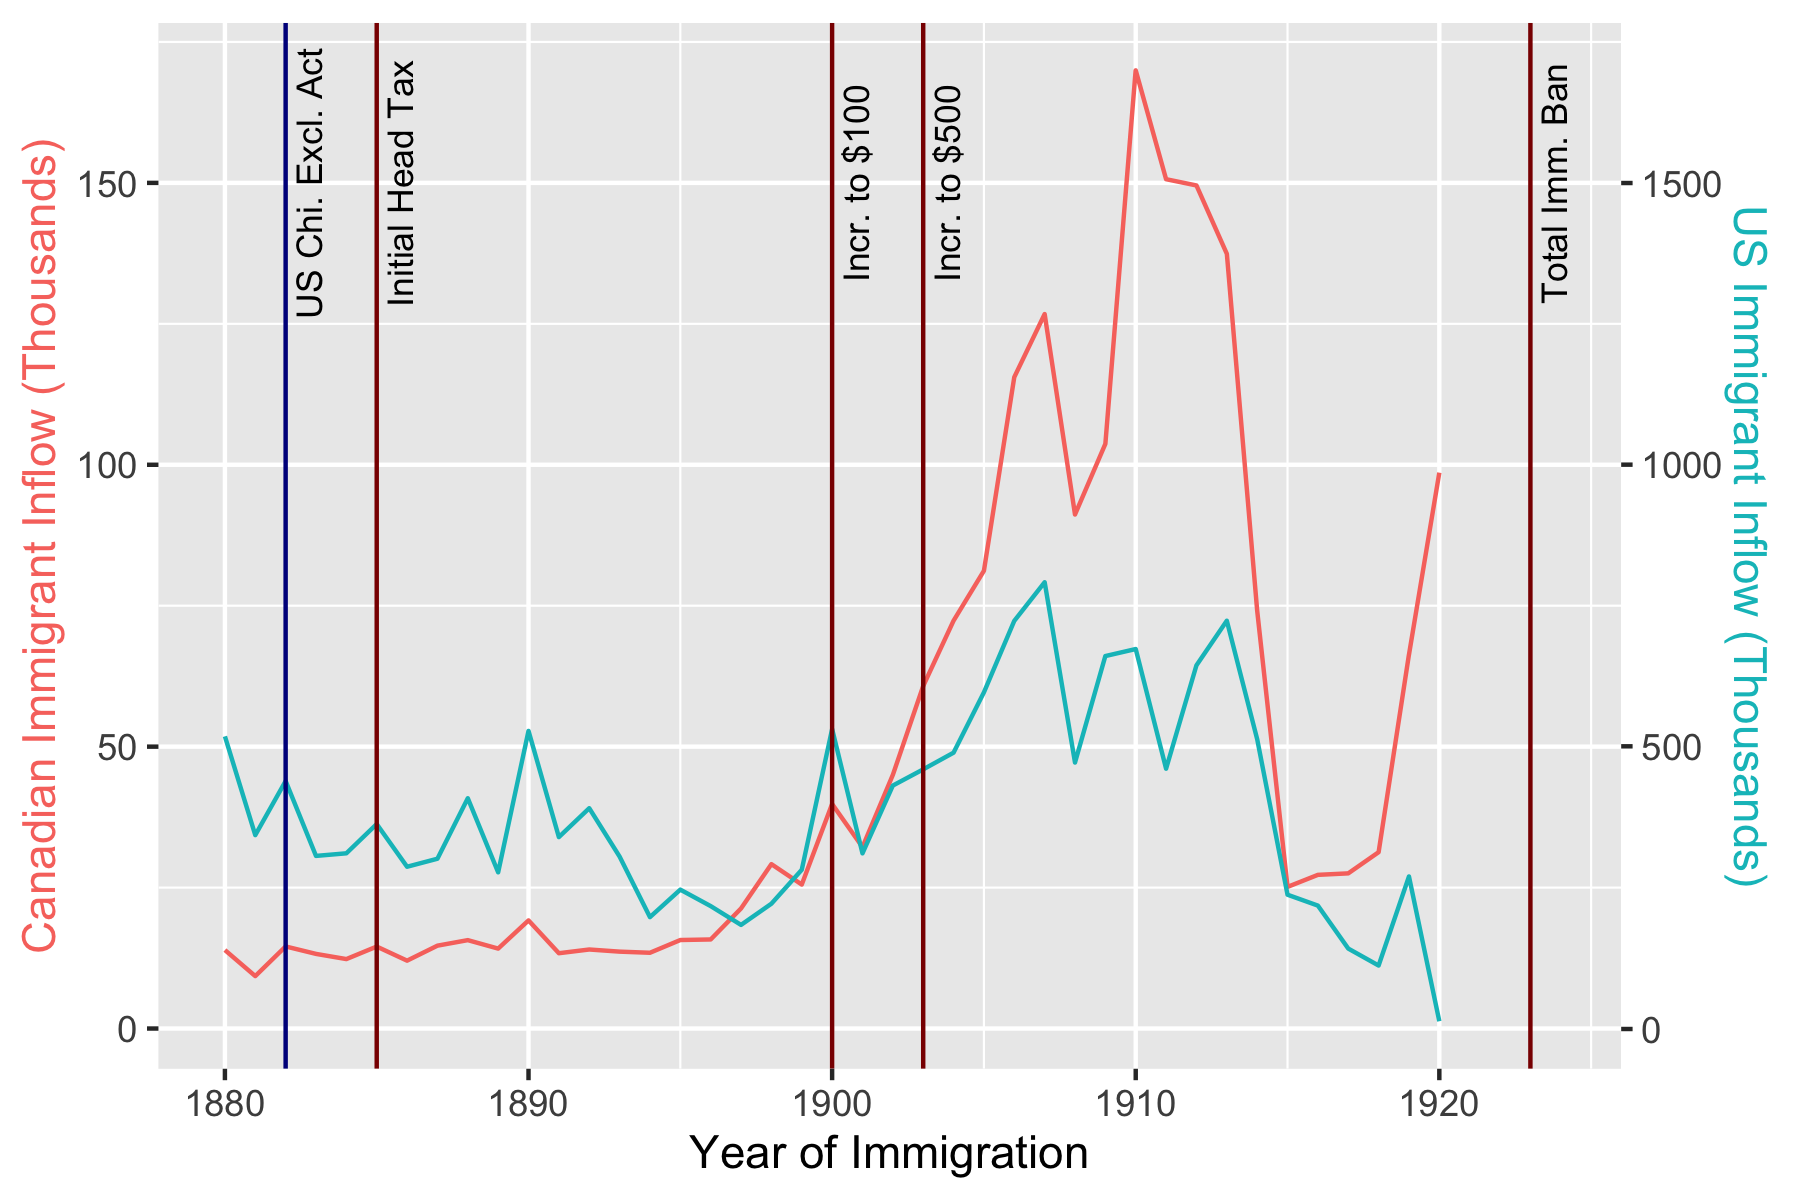
\includegraphics[width=0.9\textwidth]{../../figs/yrimm_us.png}
		\end{center}
	\end{figure}
    \hyperlink{yrimmchius}{\beamerbutton{Back to Chinese Imm. to CA/US}}
\end{frame}

%---------------------------
%  Immigration to Canada by Year by Country
%---------------------------
\begin{frame}[label = yrimmall]
	\frametitle{Immigration to Canada by Year by Country}
    \centering
	\begin{figure}[H]
		\begin{center}
			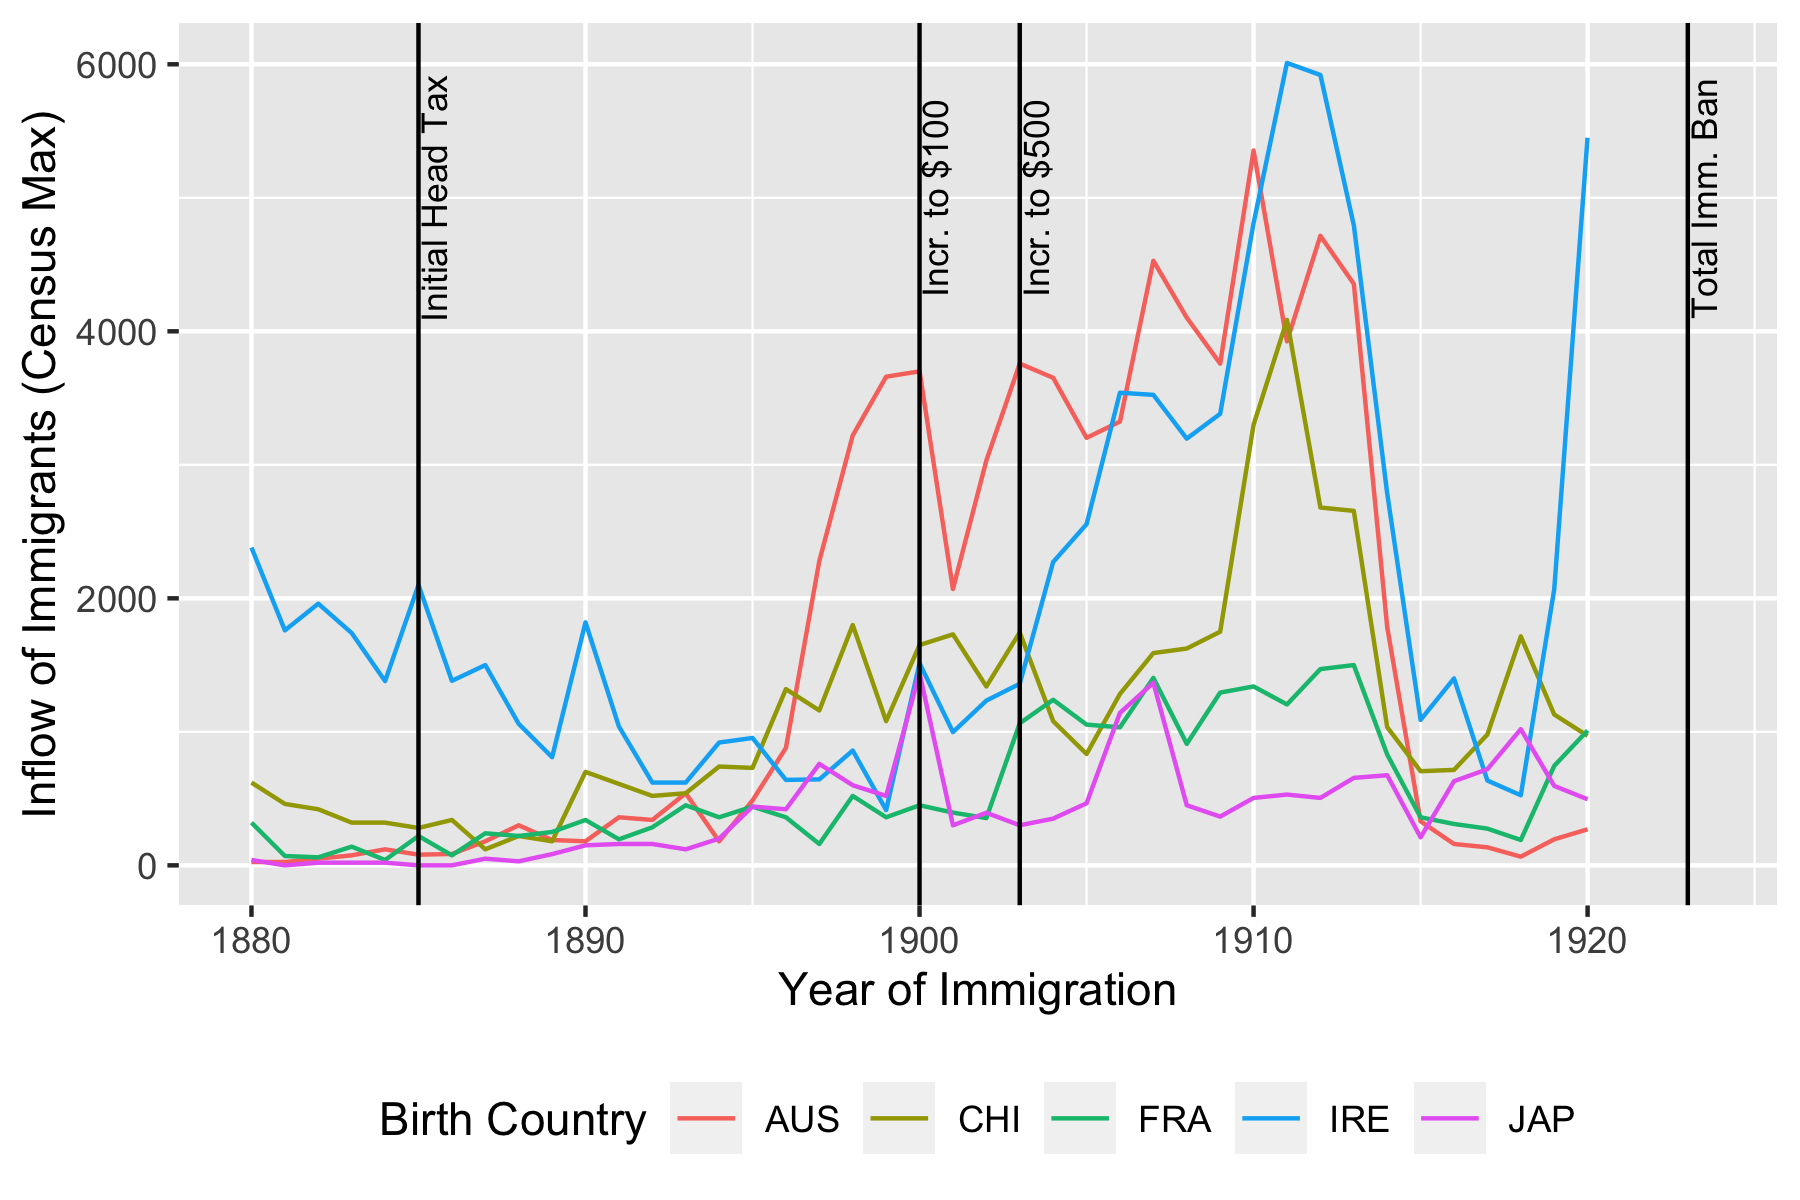
\includegraphics[width=\textwidth]{../../figs/yrimmall.png}
		\end{center}
	\end{figure}
\end{frame}
\end{document}